\part{Expression des besoins}

Étape de l’élaboration du dossier d'expression des besoins (conformément au dossier d’initialisation) : 

Le dossier d’expression des besoins contient plusieurs sous-dossiers : 
\begin{itemize}
\item Etude de l’existant, à savoir l’analyse des processus qui permettent aujourd’hui de gérer les contrats de maintenance. Le but de cette partie est donc d’avoir une vision critique de l’existant afin d’émettre un diagnostic dans l’optique de proposer une solution apportant une avancée par rapport à ce qui existe déjà.
\item Dégager les processus principaux ainsi que des objets métiers.
\item Étude de l’existant.
\item Benchmarking.
\item Élaboration de la cible fonctionnelle.
\item Définition des thèmes de progrès (s’il en est).
\end{itemize}

Avant de citer les différents éléments qui permettent de gérer les contrats de maintenance chez SPIE. Nous allons décrire les activités de SPIE dans une première partie, nous nous concentrerons notamment au niveau de SPIE Sud-Est.

\section{Etude de l'existant}

\subsection{Activités de SPIE}

Rappel de l’existant au niveau de SPIE Sud-Est :

SPIE Sud-Est est structuré en 3 directions de spécialité qui dépendent de la direction générale :

\begin{itemize}
\item Génie climatique.
\item Industries.
\item Systèmes d’informations et transport.
\end{itemize}

SPIE Sud-Est est divisé en 7 directions opérationnelles : une direction opérationnelle étant un découpage géographique au sein de la région SPIE Sud-Est. De manière synthétique, SPIE Sud-Est est donc présent dans les 3 grandes régions Rhône Alpes, Auvergne et PACA mais aussi en Suisse. SPIE Sud-Est répond aux besoins de plus de 5000 clients.

% Carte représentant le découpage géographique de SPIE.
%TODO : Vérifier l'apparence de ce visuel.
\begin {center}
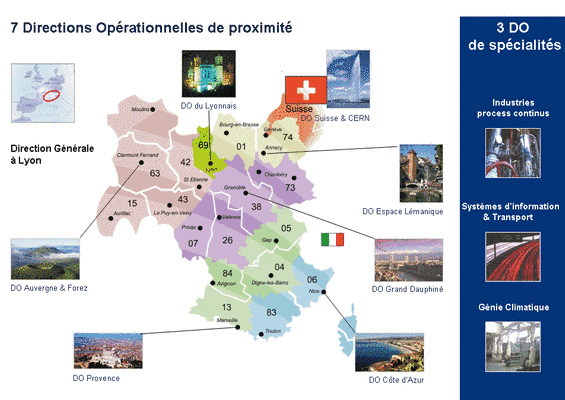
\includegraphics[width=\textwidth]{png_generaux/TerritoireSPIE.jpg}
\end {center}

Concevoir, Réaliser et Maintenir sont les 3 activités principales de l’entreprise, en appliquant ces services aux 3 domaines cités ci-dessus SPIE Sud-Est mènent des projets que l’on retrouve au sein de nos collectivités, par exemple :

Dans le domaine des transports, la mise en place des réseaux Cité, PrioCité, Vigicité, Sylvie, des sytèmes permettant de gérer et de piloter les transports en communs mais aussi de réguler la circulation au sein d’une agglomération.

Dans le domaine de la gestion de l’énergie, la mise en place de Spielum, un système gérant l’éclairage public qui rend l’éclairage plus efficace et sa consommation moindre.

Dans le domaine écologique, la mise en place de projet de grande envergure de production d’énergie “verte” (photovoltaïque, hydroélectrique...).

A travers ses projets pour les réseaux de transports en commun, SPIE dispose d’une sérieuse expérience dans les domaines du SAEIV à savoir les Systèmes d’Aide à l’Exploitation et à l’Information des Voyageurs. Ceci permet donc de répondre aux attentes des utilisateurs en ce qui concerne :

\begin{itemize}
\item l’information au voyageur (embarqué, sol et internet),
\item la supervision et régulation en temps réel du réseau,
\item l’évaluation et l'aide à l’exploitation en temps différé.
\end{itemize}

Les systèmes d’informations, souvent nécessaire aux développements des projets que SPIE met en place, sont conçus et développés au sein du département Système d’Information par 150 personnes dont 110 permanentes et représentent 18 M\euro de CA. Le travail est réparti en 3 plates-formes de développement sur Lyon, Aix-en-Provence et Vallauris.

Ce département assure la conception, le développement, l’intégration, et la mise en service des systèmes automatisés de production, des systèmes de traitement de l’Information, des solutions d’administration des systèmes et des prestations associées (Garantie, Formation, Soutien après Vente).\footnotemark

\footnotetext{Source : diapositives de Mr. JM. Berthault.}

Voici une liste des filiales de SPIE Sud-Est dans les domaines du service industriel\footnotemark :

\begin{itemize}
\item GMS : services de maintenance et prestations mécaniques en Savoie et en Isère.
\item ACEM : services industriels en Auvergne.
\item C-TRAM : services industriels dans la région lyonnaise.
\item SOMELEC : services industriels en région provençale, spécialiste des services à l’industrie agroalimentaire.
\item DCCS en Grand Dauphiné, spécialiste des systèmes de sécurité, vidéosurveillance et autres courants faibles.
\item Entreprise J. POLAUD, spécialiste des travaux extérieurs en Savoie et Nord Isère.
\item PIER : services à destination des opérateurs télécom.
\item GB Analyse : spécialiste en Analyse industrielle pour l’industrie pétrochimique (maintenance et travaux clés en main dans le domaine des systèmes d’échantillonnage d’analyse).
\item ELECTROTECH : spécialiste du génie électrique en Suisse.
\end{itemize}

\footnotetext{Source : site internet SPIE Sud-Est - http://j.mp/xTveeD}
%http://www.spie.com/a-propos-de-spie2/spie-dans-le-monde1/spie-sud-est1.html#c3771

Gestion des contrats de maintenance chez SPIE
Le processus de maintenance chez SPIE (traduction de la présentation) :
Voici un diagramme représentant l'organisation de l'entreprise SPIE. SPIE est donc organisé selon deux principes généraux, à savoir les directions de proximité (comme celle de SPIE Sud-Est) couplées à des directions techniques spécifiques. Comme il est spécifié dans les documents de processus, SPIE Sud-Est va donc faire appel au Responsable d'activités maintenance afin d'avoir l'expertise technique nécessaire dans la domaine spécifique de la maintenance concernée.

% Diagramme organisationnel de SPIE Sud-Est.
\begin {center}
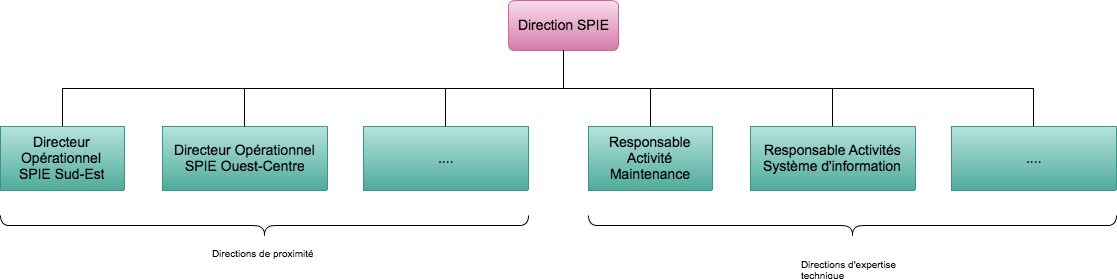
\includegraphics[width=\textwidth]{png_generaux/DiagrammeOrganisationnelSPIE.png}
\end {center}

\paragraph{Les intervenants}

\begin{itemize}
\item Le pilote de l'offre : c'est l'acteur qui sera chargé de gérer la réponse à l'appel d'offre du client. Il ménera la validation interne de l'élaboration de l'offre et sera l'intermédiaire avec le client pour répondre aux éventuelles évolutions de spécifications du client.
\item Le responsable du contrat : c’est la personne qui assure la gestion contractuelle et le reporting, le reporting est, de manière francisée, l’établissement de compte rendu remis aux supérieurs et permettant d’effectuer un bilan du projet à un moment précis de son cycle de vie (à l’issue de la réalisation d’une phase ou à la remise d’un livrable par exemple). Dans le cadre de la gestion des contrats de mainteance, on nommera un responsable d'affaire (RA) chargé de suivre le projet.
\item Le Responsable d'activité maintenace : c'est la personne qui représente une direction d'expertise technique. Le RAM sera donc l'acteur vers lequel il faudra se tourner afin de statuer sur la possibilité de réalisation de telle ou telle solution technique.
\item Le technicien de maintenance : c’est la personne (ou le groupe d’intervention) qui va intervenir sur le terrain afin d'effectuer l’acte de maintenance à proprement parler. Lui aussi est astreint à effectuer un acte de reporting auprès de son responsable afin de l'informer des difficultés et/ou solutions apportées à l’installation à maintenir. Dans le cadre de son travail d’expertise, il devra aussi informer de la nécessité d’approvisionnement en tel ou tel matériel. Exemple classique : changement d’ampoule, ajout d'équipement (e.g. de siège pour un arrêt de bus), etc.
\item Le contrôle de gestion : permet de valider ou non le reporting du responsable de contrat. La ressource en charge du contrôle de gestion ne se limite pas à la vérification pure et simple du compte rendu mais vérifie aussi qu'il assure la performance économique de l’entreprise.
\end{itemize}

% TODO: Vérifier -> La ressource ? Ca se dit ça ?

\paragraph{Le contrat}
Voici un schéma récapitulant les étapes clefs du suivie du contrat de maintenance chez SPIE :

% Processus de maintenance simplifié SPIE.
\begin {center}

\includegraphics[width=\textwidth]{png_generaux/SimplificationProcessusDeMaintenanceSPIE1.png}
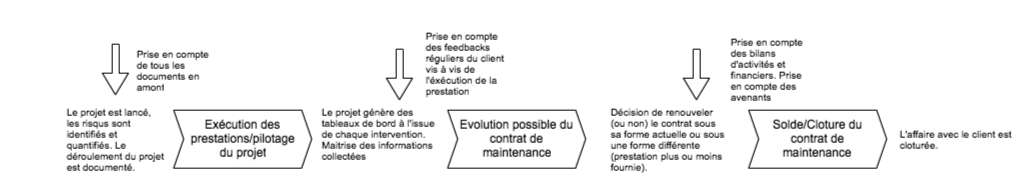
\includegraphics[width=\textwidth]{png_generaux/SimplificationProcessusDeMaintenanceSPIE2.png}
\end {center}

On distingue deux modes de fonctionnement pour l’établissement du contrat de maintenance :

\begin{itemize}
\item Partie forfaitaire : SPIE fournit une sorte de pack de maintenance, qui prévoit un éventail d’actes compris dans le forfait. Un document répertorie donc les choses pour lesquelles le client est couvert. Les tarifs sont fixés à partir des spécificités de chaque contrat. On admet ainsi que plus la couverture est importante, plus le prix du contrat sera élevé. 
\item Partie bon de commande : cette partie permet de répondre aux interventions exceptionnelles qui peuvent avoir lieu suite à des évènement tels que du vandalisme ou encore des accidents (de la circulation, comportement dangereux de l’utilisateur, etc.). De même, si le client désire des évolutions non prévues dans le contrat, SPIE lui fait une proposition chiffrée correspondant à l'intervention.
\end{itemize}

%Commentaire des schémas pour le processus de gestion des contrats de maintenance et service: http://moodle.insa-lyon.fr/file.php/108/EXISTANT_SPIE/Processus_de_maintenance_SPIE.pdf

\begin{itemize}
\item Opportunité de contrat de service.
\item Offre et revue d’offre (X).
\item Négociation client.
\item Revue de commande (Q).
\item Lancement des prestations de service et travaux (Y).
\item Exécution des prestations et gestion (Y).%(coupé en 2 en fait).
\item Évolution du contrat (X).
\item Solde de l’affaire et du contrat (Y).
\item Fin de processus affaire Maintenance et Services.
\end{itemize}

\subsection{Processus de gestion de contrat de maintenance}

\subsubsection{Offre et revue d’offre}

Ce sous-processus peut débuter suite à un processus commercial. Le processus commercial peut consister en une prospection chez des clients ciblés et susceptibles d’être intéressés par la mise en place d’un contrat de maintenance. Ceci suppose donc que SPIE n’ait pas forcément conçu et réalisé le système que le client cherche à maintenir. L’offre/revue d’offre peut de même débuter un processus travaux. Ici, la contraction d’un contrat de maintenance par un client est la suite logique de la réalisation d’un projet. Après avoir réalisé un projet complexe, SPIE propose à son client le contrat de maintenance qui fera office de ``garantie payante'' sur le système mis en place.

La réponse à un appel d’offre donne lieux à une opportunité de contrat de service. Le RA (Responsable d’affaire) et le RAM (Responsable d’activité maintenance) décident en fonction des données clients, du climat concurrentiel et des opportunités de clients si une étude sera faite ou non, avec la participation du DO (Directeur Operationnel) et du COM (Commercial). Dans tous les cas, un PO (Pilote de l’offre) est désigné.

Si la réponse est négative, une confirmation de non-réponse est envoyée au client sous la forme d’un courrier type, sous la responsabilité du PO.

Si la réponse est positive, une collecte de données est effectuée en suivant un protocole précis. Ces données sont ensuite analysées et donnent lieu à un rapport d’analyse des risques (juridiques, techniques, commerciaux, financiers, environnementaux, etc.) produit par les acteurs ayant les compétences requises (MAR, Ressources Humaines, Service Moyens, Service Achats, Service Juridique, Direction QSE). Cette analyse de risques et de faisabilité permet de donner une réponse au client quant à l'avenir de l’offre.

Après une réponse positive (SPIE Sud-Est va donc répondre à l’opportunité d’offre), une procédure administrative va initialiser le processus d'offre. Cela va permettre d'enregistrer le dossier d'étude. Le dossier de réponse sera établi conformément au réglement de consultation.

Il va ensuite falloir donner des propositions de solutions chiffrées sous forme de fiches de calcul des déboursés et de fiches devis, cela en se basant sur les coûts induits lors de la réalisation d'actes de maintenance antérieurs (utilisation des contrats chiffrés précédents).

Après prise de décision de la part du RAM/DO/RA, une solution est sélectionnée et son prix est validé, la fiche du devis retenu est alors signée.

L'offre est rédigée, avec entre autre la définition des conditions générales de vente des prestations de services. Elle est ensuite validée en interne par le DO, le RAM, le RA et le COM, (toujours sous la responsabilité du PO), avant d’être transmise dans les délais au client, avec un courrier d'accompagnement. Une preuve d'envoi de cette offre est conservée.

\subsubsection{Négociation client}

Après la réception de l’offre par le client, celui-ci renvoie ses impressions et les modifications qu'il souhaite apporter à l'offre proposée par SPIE. Il se peut que certains points doivent être éclaircis afin que la maîtrise d'oeuvre et la maîtrise d'ouvrage aient la même idée du projet final.

\subsubsection{Revue de commande}

A l'issue de la phase de négociation avec le client, l'offre est dite validée, et la commande est donc enregistrée dans le SI. Commence alors la phase de diffusion de la commande, celle-ci va être transmise aux différents services de SPIE Sud-Est afin d’en informer les acteurs principaux. Puisque la commande est lancée, on décide d'y assigner un PO, ou pilote de l’offre, chargé de mener la mise en place de la prestation de services. On convoque ensuite une commission de revue de commande permettant de chiffrer les écarts entre l'offre originale proposée par SPIE et les modifications apportées par le client. Cette phase permet de matérialiser l'offre en une commande précise qui cette fois répond aux attentes du client. Cette commande alors validée par SPIE Sud-Est est re-soumise au client afin qu'il puisse y apporter d'ultimes modifications. Ce retour chez le client permet une fois de plus de préciser les exigences de celui-ci vis à vis du contrat de maintenance en lui-même. Lorsque cette commande est validée par le client et par SPIE Sud-Est, le contrat est référencé et la prestation de service est prête à être lancée.

\subsubsection{Lancement des prestations de service et travaux}

Lorsqu'une commande est acceptée et que les spécifications client sont connues, on s'attache à la réalisation du dossier complet en prenant en compte les données internes (QSE, gestion, RH), le dossier contractuel et le dossier d'étude fait par le RA. Une attention particulière est apportée à la création du dossier d'affaire. Ceci clos la partie amont de la réalisation.

Le dossier complet est ensuite analysé en terme d'exigences et besoins du projet. Ceci permet l'identification et la nomination des acteurs sous la forme d'un organigramme contractuel.

Une fois la liste des ressources à mobiliser, le dossier de synthèse des exigences et l'organigramme contractuels finalisés, l'équipe se retrouve pour la réunion de lancement. Cette réunion sert à définir les prestations de services et travaux, et c'est l'occasion d'établir un plan d'action par acteur, permettant la mobilisation des ressouces\footnotemark.

\footnotetext{La conformité de l'habilitation et la formation des ressources devra être vérifiée}

Il s’agit ensuite de créer les procédures et documents opérationnels à partir du dossier de synthèse et des spécifications client. Une fois compilées, ces données permettent de mettre en place une procédure de prise en charge, un plan de maintenance initial, et selon les besoins exprimés, un plan d’assurance qualité et/ou un plan de prévention.

Les exigences contractuelles et les règles de la filiale permettent d'initialiser les systèmes de gestion (financière et technique). Il s'agit ensuite d'établir un rapport d'état des lieux en prenant en compte les documents et installations client.

La prise en charge peut alors avoir lieu, car la situation initiale est connue et maîtrisée. Ceci donne lieu à un PV de prise en charge, comportant des informations sur l'état des installations, du matériel et de la logistique.

La réalisation peut alors enfin commencer.

\subsubsection{Réalisation des prestations de maintenance}

A la lecture du cahier des charges des travaux client, la décision est prise de donner suite, ou non, à la réalisation de prestations de maintenance. Si c'est le cas, l'analyse des travaux induits va entraîner. Si ceux-ci s'avèrent légers, les dossiers vont être transmis à l'entité travaux. Dans le cas contraire, il va falloir les chiffrer et les valider, pour enfin envoyer un devis au client conformément aux clauses contractuelles prévues.

Une fois les consignes nécéssaires transmises au responsable d'exécution, les travaux vont être préparés en fonction du cahier des charges. Les documents concernés seront mis à jour au fur et à mesure de la réalisation des prestations. Une fois les prestations terminées, le service marché envoi la facture au client.

\subsubsection{Évolution du contrat}

Suite à la réalisation, et après analyse du tableau de bord de l'affaire et des activités, des données comptables et en prenant en compte les orientations client et interne, la décision est prise conjointement par le client, le DO, le RA, la QSE, le JUR, le ROC, ceci sous la responsabilité du RAM, de renouveler ou non le contrat de maintenance, sous sa forme initiale, ou sous une nouvelle forme renégociée.

\subsubsection{Solde de l’affaire et du contrat}

Le processus de gestion se termine par la revue de fin d'affaire. C'est ensuite que les prestations et les travaux sont soldés. Nous pouvons maintenant mettre fin au processus affaire ``Maintenance et Services''.

\subsection{Applications utilisées chez SPIE}

Plusieurs applications sont utilisées par SPIE pour la gestion des contrats :

\begin{itemize}
\item RHI/Ndf (gestion des heures) : ce logiciel permet de prévoir et de suivre les heures et les frais correspondant à une intervention.
\item ADA/ADM (achat/moyen) : cette application permet la commande au fournisseur de tous les éléments nécessaire à une intervention.
\item ADV (administration des ventes) : lie la commande à un contrat. Permet de contrôler l’état de chaque contrat.
\item SUPRA (gestion des affaires) : création des nouveaux contrats de maintenance.
\end{itemize}

% TODO: Reformuler.
On distingue la gestion des contrats de maintenance de la gestion des contrats de services :

\begin{itemize}
\item La gestion des contrats de maintenance se focalise sur la correction et la prévention systématique et prévisionnelle des travaux. Elle regroupe souvent aussi des fonctionnalités ouvertes à des utilisateurs au-delà du service de maintenance, comme les demandes d’interventions permettant aux personnes autorisées de signaler une anomalie à prendre en compte dans la maintenance.
\item La gestion des contrats de service s’occupe de maintenir ou rétablir un bien dans un état spécifié afin que celui-ci soit en mesure d’assurer un service déterminé.
\end{itemize}

\section{Benchmarking}

Cette partie fait suite à l'analyse du système existant, de la mise en relief de ses dysfonctionnements et donc des axes de progrès. Nous allons maintenant chercher des renseignements sur les bonnes pratiques mises en place par des organisations externes reconnues, pour s'inspirer des modèles, normes et processus courants afin de considérer leur application à SPIE.

\subsection{MySAP}

Nos recherches porteront sur les trois solutions suivantes :

\begin{itemize}
\item SAP Crystal Solutions
\item SAP BusinessObjects BI OnDemand
\item SAP BusinessObjects Edge Solutions
\end{itemize}

L'objectif est de détailler les avantages de chacune de ces solutions, puis d'indiquer dans quelle mesure elles sont adaptées à l’entreprise SPIE.

\subsection{SAP Crystal Solutions}

Cette solution mySAP offre un rapport complet des solutions de conception et de gestion pour les petites entreprises et les directions fonctionnelles. Elle permet un meilleur ajustement pour les entreprises qui ont besoin de rapports puissants avec accès à toute source de données, et un besoin de fonctionnalités pour la visualisation, la gestion, le partage et la distribution. Enfin, c’est idéal pour produire des rapports et des tableaux de bord.

Cette solution a des milliers de partenaires dans tous les secteurs et dans 80 pays, ce qui assure sa généricité.

Elle est disponible en 16 langues, ce qui pour l’instant n’est pas extrêmement pertinent pour SPIE, mais cela pourrait le devenir s’ils s’internationalisent davantage.

C’est une solution particulièrement adaptée pour des entreprises de 10 à 500 employés, ou plus.
Le temps de mise en oeuvre peut aller de un à 8 jours. L’usage d’un expert certifié SAP est recommandé pour une mise en oeuvre plus rapide.

En terme d’IT (Information Technology department), il est nécessaire d’avoir au moins un minimum de ressources. Il est possible de mettre cette plateforme en place sur site, par hébergement, sur la demande, et par “desktop deployment”.

Le tout n’est pas extrêmement onéreux: les prix partent de 479 euros.

\subsection{SAP BusinessObjects BI OnDemand}

Cette solution sous forme de Software-as-a-service (SaaS) est complete et intuitive. Elle est particulièrement adaptée aux entreprises qui ont besoin d’une solution complète de BI (Business Intelligence) pour traverser les possibilités SAP, pour obtenir des rapports et partager des données qui fournissent un aperçu rapide des bilans. Elle promet de réduire le fardeau sur les IT.

Du point de vue partenarial, cette solution a des milliers de partenaires répartis dans tous les secteurs et dans 80 pays.

Cette solution n’est disponible qu’en anglais.

Cela s’adresse davantage à des entreprises comptabilisant de un à cinq mille employés, ou plus.

Un avantage certain de cette solution par rapport à celle présentée précédemment est son temps de mise en oeuvre, qui est typiquement immédiat et sans douleur.

L’approche IT utilisée est à la demande (dans la mesure où il  s'agit d’un SaaS).

Le prix se fait par abonnement mensuel (ce qui est probablement moins cher). C’est un prix qui dépend des différents modules SAP BusinessObjects BI OnDemand choisi par l’entreprise et intégrés les uns aux autres.

\subsection{SAP BusinessObjects Edge Solutions}

Cette solution extrêmement complète de BI (Business Intelligence) permet une bonne gestion de l’information et fournit des logiciels de gestion de la performance, en particulier pour les moyennes entreprises.

C’est une solution idéale pour les entreprises qui ont besoin de toutes les possibilités en matière de reporting d’entreprises, de requêtes ad hoc et d’analyse business. Cette solution fournit des tableaux de bord, des outils de visualisation, une gestion des données flexible, des outils de planification et de budgétisation de la stratégie comme de la gestion.

Derechef, des millers de partenaires dans tous les secteurs et dans 80 pays apportent leur soutien à cette solution.

Elle est disponible en 12 languages.

C’est une offre particulièrement adaptée à des entreprises de cent à deux mille cinq cent employés. La mise en oeuvre se fait en quatre à huit semaines.

Elle nécessite un minimum de ressources IT: un hébergement est requis afin de permettre un accès par site Internet.

La license traditionnelle pour cette solution est de 8000 euros pour 10 utilisateurs.

\subsection{Concurrence}

L’objectif est de se positionner vis-à-vis de la concurrence, à savoir principalement Bouygues, Eifface,Vinci, en trouvant des indicateurs qui permettrait d’évaluer les performances de chacun pour ensuite trouver les points forts au niveau des processus, pour s’en inspirer.

Malheureusement, il est difficile de trouver les informations utiles sur Internet, la plus plupart des informations étant uniquement commerciales, pour des raisons de confidentialité, le détails des processus, les délais, les coûts ne sont accessible au public. De plus, les indicateurs publics (chiffre d’affaires, résultat nets) ne sont pas assez détaillés pour nous permettre de situer Spie par rapport à la concurrence. Avoir la marge nette sur le secteur de la maintenance aurait pourtant été un indicateur intéressant.

Il faudrait donc disposer de plus de temps et de sources d'informations autre qu'Internet pour que avoir un vrai comparatif de la concurrence et obtenir des détails sur leurs processus métiers.

\subsection{Autres solutions logicielles}

L’objectif est de comparer d’autres solutions logicielles existantes, spécialisées dans la gestion de la maintenance afin de trouver des éléments qui pourrait apporter un plus à SPIE.

On a sélectionné plusieurs progiciels spécialisé dans la gestion de maintenance reconnu et utilisé par de nombreuses entreprise. Nos informations proviennent de leur site web:

Carl Software\footnotemark
Optimaint\footnotemark

% Site internet : http://www.carl-software.fr
\footnotetext{Site internet Carl Software : http://j.mp/carl-software}
% Site internet : http://www.europrint-gmao.fr
\footnotetext{Site internet Optimaint : http://j.mp/europrint}

Malheureusement, ces sites ne sont que des vitrines et peu d’informations sur le fond sont disponibles. De même que pour le benchmarking de la concurrence, on ne pourra pas espérer apprendre de bonnes pratiques, ni comment sont gérés les processus. On se contentera de dégager les fonctionnalités communes et importantes pour la gestion de la maintenance.

Les principales fonctionnalités sont :

\begin{itemize}
\item le tableau de bord,
\item les demandes d’interventions,
\item les fiches d'équipement et de suivi,
\item le suivi des interventions,
\item le suivi des stocks,
\item le suivi des achats,
\item le suivi des budgets,
\item le suivi des projets d’investissements,
\item le suivi des contrats sous-traitants,
\item et l'analyse des temps et des coûts.
\end{itemize}

\section{Elaboration de la cible fonctionnelle}
Dans l'ensemble des processus de gestion des contrats de maintenance, nous avons mis en avant des entités organisationnelles précisent qui interviennent chacune à leur façon dans l'évolution du contrat.

\subsection{Definition du Modele d'Activité} 

\begin{itemize}
\item Gérer l'appel d'offre : étude de l'appel d'offre en interne. Cette étape est dirigée par le pilote de l'offre, elle va donc permettre de proposer l'ébauche de la solution que SPIE peut apporter au client en terme de contrats de maintenance.
\item Gérer la commande : lorsque l'appel d'offre a été validé et que le client a parfaitement définit ses besoins au niveau du contrat de maintenance, SPIE est à même de lancer la \og commande \fg du contrat de maintenance. L'équipe de travail examinera donc les ressources humaines et matérielles à mettre en place pour honorer le contrat suivant les exigences formulées par le client.
\item Gérer l'activité de maintenance : le responsable d'activité maintenance (RAM) au sein de SPIE garde un oeil sur l'avancée de la maintenance. Le RAM peut donc adapter la manière dont les techniciens vont intervenir sur les zones à maintenir afin de respecter les processus de maintenance definit par SPIE. Le service RH organisera la répartition des ressources humaines (technicien) qui seront en charge de l'intervention direct sur site.
\item Gérer la prestation de service : c'est l'activité du responsable d'affaire d'évaluer le déroulement du contrat. Le RA capitalise donc les informations venant de tous les acteurs du contrat de maintenance. En synthétisant toutes ces informations (reporting) et en gardant en tête les risques et les échéances, il doit être capable de déterminer les perspectives d'évolution du contrat.
\item Gérer l'évolution du contrat : en fonction du déroulement de la prestation de service mais aussi de la réalisation éventuelle de certains risques (surcoût, retard…), les acteurs clefs du projet (RAM, RA, service financier) vont faire évoluer le projet. Par exemple, si la prestation se passe bien, il pourra être proposé au client d'étendre ce contrat de maintenance à d'autres de ces installations. Si la prestation de service sort du cadre établi lors de l'appel d'offre, on établira alors des avenants.
\item Gérer la facturation : à l'issue de chaque phase clef du projet, il faudra formaliser les procédures de recettes. 
\end{itemize}

Voici un modèle d'activité synthétique pour la gestion des contrats de maintenance chez SPIE :

\begin {center}
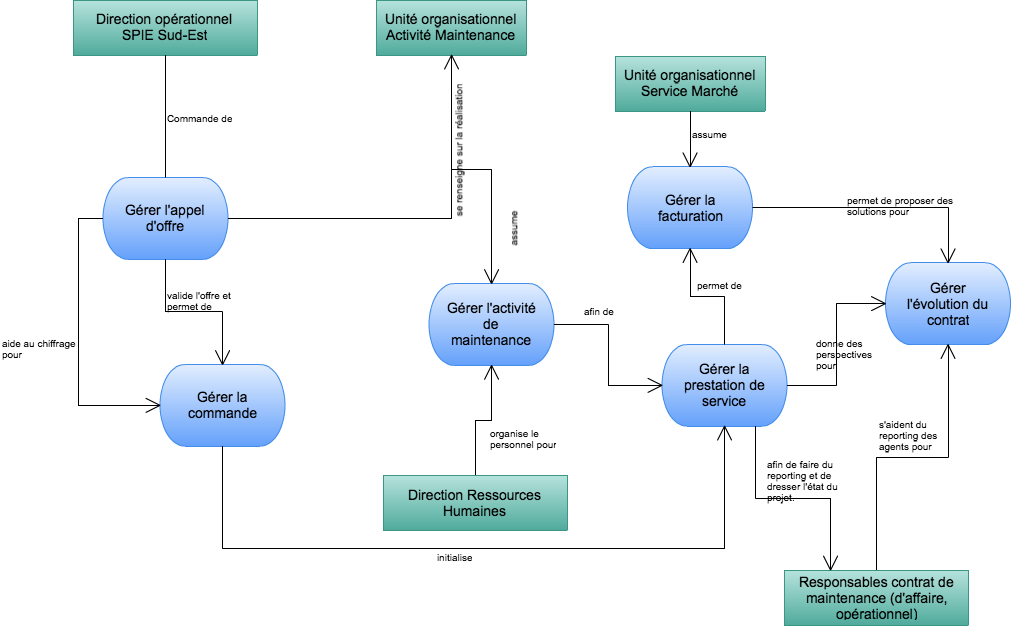
\includegraphics[width=\textwidth]{png_generaux/DiagrammeModeleActivite.png}
\end {center}

\subsection{Modèle Conceptuel des traitement} 
Vis à vis des documents fournis par SPIE, nous disposons déjà de descriptions formalisées des processus métier dans le cadre de la gestion des contrats de maintenance chez SPIE. Il nous semble donc inutile de retraduire ces processus déjà assez précis.

Il est cependant possible d'effectuer des critiques sur la manière dont les processus s'imbriquent :

\begin{itemize}
\item Le reporting du technicien de maintenance n'est, selon nous, pas assez détaillé. En effet, il serait fortement intéressant de plus faire participer le techniciens à la rédaction, brève bien entendu, d'un rapport d'intervention qui serait concilié au sein du SI afin que son diagnostic puisse être réutilisé. Dans la même idée, il serait intéressant d'affilier un technicien (ou groupe de technicien) toujours au même chantier de maintenance. Cette tactique permet ainsi au technicien de connaître parfaitement son domaine d'intervention et ainsi de minimiser le coût humain.
\item Enrichir le SI de rapports d'interventions permettrait de capitaliser et de gagner de l'expérience dans le domaine de l'expertise, un des domaines phare de SPIE.
\item Formaliser les éventuels problèmes juridiques. Un contrat avorte souvent du fait de l'incompréhension entre la MOA et la MOE. Dans les diagrammes de processus qui nous sont fournis, il pourrait être pertinent d'ajouter un processus gestion des contentieux. De même, ce processus pourrait permettre d'enrichir le SI en expérience sur le déroulement des contrats.
\end{itemize}


\subsection{Diagramme de cas d'utilisation de l'existant}
Il est cependant utile d'établir des diagrammes de cas d'utilisation afin de définir avec plus de précisions les notions présentes dans le modèle d'activité. Voici donc les diagrammes de cas d'utilisation correspondant à chacunes des étapes clefs de la gestion des contrats de maintenance chez SPIE.

\begin {center}
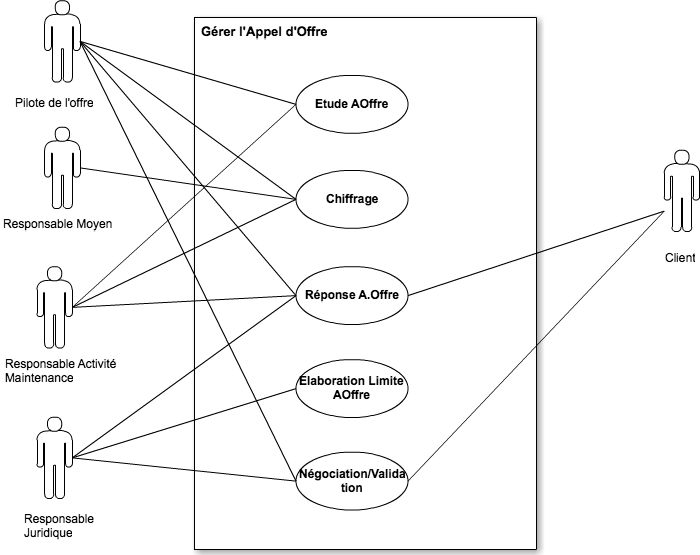
\includegraphics[width=\textwidth]{png_generaux/DCUAppelOffre.png}
\end {center}

\begin {center}
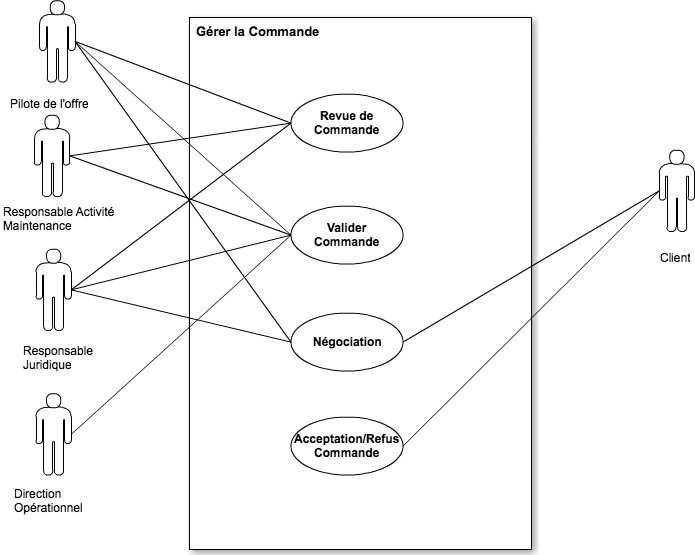
\includegraphics[width=\textwidth]{png_generaux/DCUGererCommande.png}
\end {center}

\begin {center}
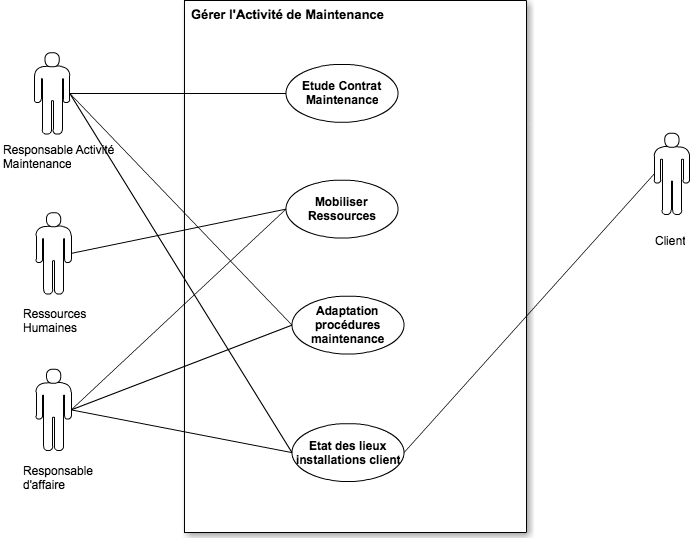
\includegraphics[width=\textwidth]{png_generaux/DCUGererActiMaintenance.png}
\end {center}

\begin {center}
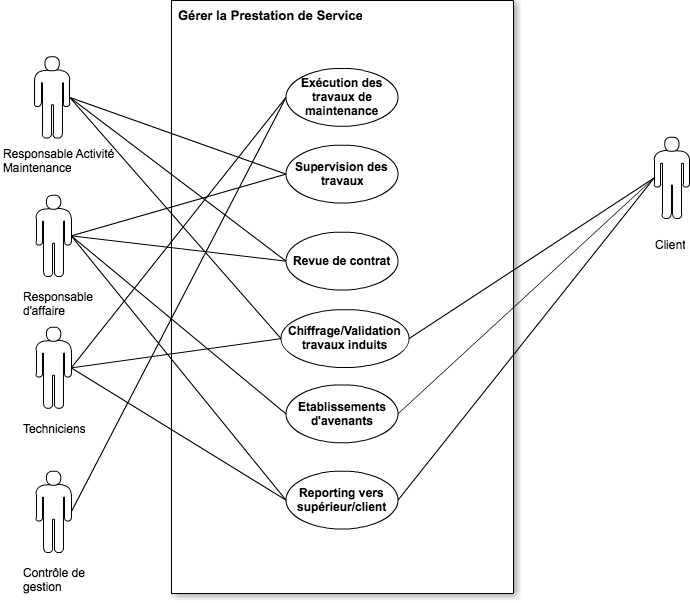
\includegraphics[width=\textwidth]{png_generaux/DCUGererPrestationService.png}
\end {center}

\begin {center}
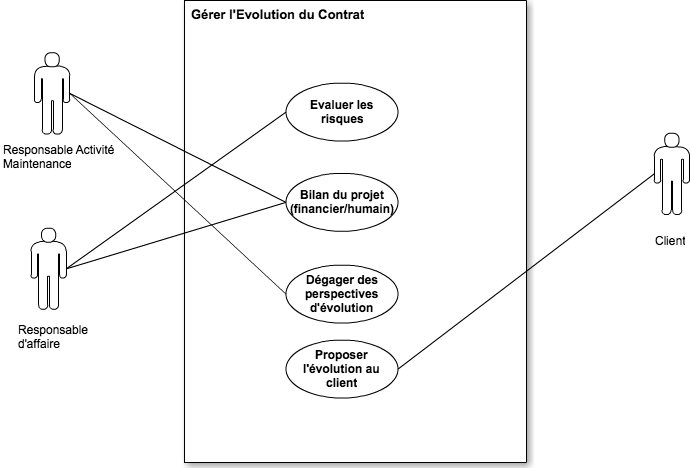
\includegraphics[width=\textwidth]{png_generaux/DCUGererEvolutionContrat.png}
\end {center}

\begin {center}
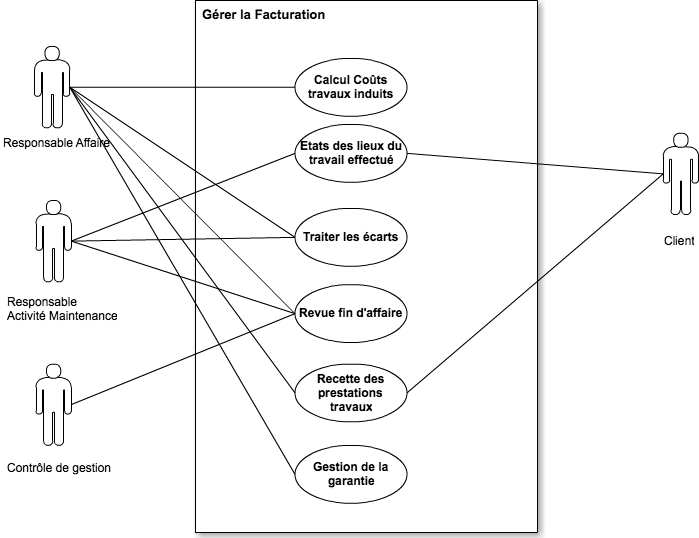
\includegraphics[width=\textwidth]{png_generaux/DCUGererFacturation.png}
\end {center}

\subsection{Diagrammes de processus contenant les axes d'amélioration}

\section{Définition des axes de progrès}

Les processus détaillés dans les documents annexes fonctionnent le plus souvent en parallèle et sur des applications informatiques différentes. Il en résulte que souvent, les différentes unités organisationnelles ne sont pas en accord sur certains points. Le but principal de cette étude est donc de regrouper l'ensemble des procédures de gestion des contrats de maintenance au sein d'un même système d'information ou chaque unité organisationnelle aurait son rôle. Cette interface unique va ainsi permettre de créer un référentiel commun de travail entre toutes les équipes qui gravitent autour du domaine d'expertise maintenance. 

D'autres part, si l'on regarde plus précisément le processus global de gestion des contrats de maintenance, ce qu'il est important d'améliorer est sans nul doute le fait de pouvoir réutiliser l'expérience acquise par SPIE lors de la réalisation d'anciens contrats de maintenance. Cette expérience doit pouvoir être réutilisée dans toute les étapes du cycle de vie du contrat de maintenance, de la réponse à l'appel d'offre jusqu'a la rélisation technique à proprement parler.

\subsection {Les domaines d'application}
Voici les domaines d'applications des axes de progrès, pour plus de détails, vous pouvez vous référer aux diagrammes Aris présentant les modifications des processus métiers.
\begin{itemize}
\item La gestion de l'appel d'offre : consultation de la base de données à deux niveaux : tout d'abord pour l'étude de faisabilité technique, cette consultation pourra permettre de savoir si ce qui est demandé dans l'appel d'offre a déjà été réalisé par SPIE ou si cela paraît techniquement faisable au vue des contrats de maintenance déjà réalisés par l'entreprise. Ensuite, pour le chiffrage de la réponse à l'appel d'offre, il est important de prendre en compte les montants des contrats précédent. Ainsi, si l'on trouve des contrats similaires à celui que l'on est en train d'établir, il peut être intéressant de savoir quel a été son prix.
\item La mobilisation des ressources humaines : lorsque le contrat a été validé et signé par les deux parties il est important de mobiliser les bons techniciens. Notre système permettra donc de recommander des techniciens pour telle ou telle prestation de maintenance en fonction de son expérience sur ce domaine. Ceci permettra alors de laisser un technicien dans son domaine de compétence. De même ce système permettra d'envoyer toujours le même groupe de technicien pour un contrat donné.
\item La réalisation de la prestation de maintenance : s'il s'avère que l'on doive changer de technicien pour un contrat, il est nécessaire que les interventions déjà effectuées soient documentées. Ainsi après chaque intervention de la part d'un technicien, celui-ci devra remplir la base de données en conseil et en mots clefs.
\end{itemize}

\subsection {concepts généraux à mettre en place}
\begin{itemize}
\item Base de données : vis à vis de la récupération des informations liées à chaque contrat il s'agit de mettre en place une base de données qui permette de faire la jonction entre le contrat en lui même et les informations qui le concernent à savoir pour chaque processus des notes de bon/mauvais déroulement, des indications d'éventuels surcoûts, des informations concernant la relation avec le client ou encore sur le déroulement des opérations de maintenance à proprement parler. 
\item Base de connaissances : pour chaque spécialité de maintenance il sera intéressant de mettre en place des informations dans une base de connaissance afin d'automatiser autant que possible la génération des contrats de maintenance. Cette base de connaissance mettra nécessairement du temps à être utile car elle sa pertinence se base sur le grand nombre d'informations (connaissances) et de méthodes (règles) qu'elle contient.
\item Mot clefs : à l'image du réseau social twitter il sera nécessaire d'adjoindre des "tags" ou mot clefs à chaque contrat de maintenance. Il sera donc possible ensuite de rechercher des contrats de maintenance par mots clefs.
\item Moteur de recommandations : lors de la création d'un nouveau contrat de maintenance on lui adjoint des mots clefs. Afin d'aider les RA, RAM et techniciens dans le suivi de ce contrat on pourra demander l'affichage des contrats de maintenance les plus proches de celui que l'on est en train de créer. Cette recommandation sera donc une aide précieuse dans l'élaboration du chiffrage du contrat par exemple. Cette recommandation peut de même intervenir auprès du technicien lorsqu'il se rendra sur le site pour effectuer un réparation. Il lui sera en effet conseillé d'emmener tel ou tel outils spécifique ou encore de faire attention à tel ou tel paramètre en particulier.
\end{itemize}
L'idée sous jacente à la mise en place d'un tel système est de pouvoir capitaliser sur chaque contrat de maintenance et ainsi de pouvoir réutiliser les expériences passée afin de ne pas recommettre les mêmes erreurs ou encore de reproduire les pratiques qui ont menées au succés du contrat de maintenance. Ainsi, plus le système sera fourni en informations et mots clefs plus son utilité se fera sentir. Ce procédé permet aussi de \og poser les impressions sur le papier \fg et ainsi de pouvoir garder l'information de manière claire et précise.


Voici les informations qu'il faudra fournir à la base de donnée pour chaque acteur : 
\begin{itemize}
\item Le Responsable d'Affaire : A la création du contrat de maintenance dans la base de données il sera chargé (son groupe de travail) de remplir les informations et mots clefs directement liées à l'initialisation du contrat. Lors du chiffrage de l'appel d'offre, le RA devra de même renseigner les prix auxquels il a chiffrer le contrat de maintenance.
\item Le Technicien : Avant l'intervention : se renseigner via la base de connaissances sur les spécificités de l'intervention qu'il va mener. En se renseignant via l'interface Web il pourra ainsi éventuellement se rendre compte qu'un outil spécifique est nécessaire ou que ce type d'opération va prendre plus de temps que prévu.
Après l'intervention : Ecrire son bilan d'intervention via l'interface de la base de données. Ce bilan permettra alors de renseigner les prochains intervenants sur ce type d'intervention. Ceci permet donc d'enrichir la base de données via le rapport de prise en charge des agents de maintenance.
\item Le Client : L'équipe en charge du contrat devra densifié la remise de rapports au client afin d'assurer un meilleur service. La rédaction de ces rapports sera grandement facilitée grâce aux mots clefs remplis pour chaque projet. D'autre part, le client pourra être lui aussi tenu si il le souhaite de rédiger un rapport de satisfaction concernant le travail effectué dans le cadre du contrat de maintenance. Ce rapport sera lui aussi ajouté au contenu de la base de données à l'issue de la phase de recette.
\end{itemize}
Toutes ces informations devront être stockées sur un portail ou chaque intervenant du contrat de maintenance pourra aller se référer rapidement.

\subsection{Changement à apporter à l'existant}
Vis à vis du processus aujourd'hui en place pour la gestion de contrats de maintenance, des changements sont à prévoir dans l'organisation du travail. Un effort conséquent de rédaction est à faire si l'on veut que le système de recommandation soit performant. Une période de formation que nous estimons relativement courte sera nécessaire afin de familiariser les différents acteurs à l'utilisation de la base de données (via une interface web personalisée). Pour que la mise en place d'un tel système soit concluante, il faut que celle-ci ne fasse pas perdre un temps trop important par rapport à son utilité. Les RA et RAM seront donc les éléments motivateurs de la mise en place du sytème de recommandations.

A priori de nouveaux postes de travail ne sont pas à prévoir suite à la mise en place de la \og base de données intelligente \fg (voir paragraphe suivant).

\subsection{Capitalisation des expériences}
Nous distinguons deux manières principales de pouvoir tirer des bonnes pratiques de ce système :
\begin{itemize}
\item Consultation de la base de données : cette idée est exposée dans les paragraphes précédents, elle permet aux acteurs du projet de prendre connaissance de ce qui s'est déjà passé pour la gestion des contrats de maintenance chez SPIE
\item Amélioration de la gestion des contrats de maintenance : il s'agirait, dans ce cas, de créer un poste de travail (qui pourra être temporaire) et qui sera chargé d'analyser plus finement les raisons de l'échec ou de la réussite d'un projet. Cette ressource aurait donc comme objectif de tirer des enseignements des informations fournis par la base de données afin d'améliorer le processus de gestion des contrats en lui même. Cette ressource peut-être personifiée comme un consultant en processus métier. Il est évident que son intervention sera judicieuse si la base de données contient assez d'informations sur les contrats précédents.Cette ressource pourra participer à la rédaction d'un manuel de management applicable aux activités de maintenance.

\medskip

D'autre part, le fait de devoir commenter chaque phase du projet force chaque acteur à respecter le déroulement des phases assez scrupuleusement et permet ainsi à chacun de resituer le contexte du projet. Plus qu'une activité de traçage des activités concernant le projet, cela permet d'avoir une vue d'ensemble rapide de l'état de santé du contrat de maintenance. C'est donc un vrai mécanisme de suivi qui se met en place.


Ce receuil d'informations permettra dans le même temps d'effectuer une analyse des risques tout au long du projet. En prenant comme référentiel les contrats qui se sont déjà déroulés avec succès on pourra évaluer le risque en temps réel pour chaque phase. Le rapport de risque sera lui même ajouté comme \og commentaire \fg du contrat de maintenance et permettra aussi d'enrichir la base de données.

\end{itemize}
